\documentclass[twoside]{article}
\usepackage{aistats2014}
\usepackage{braket}
\usepackage[]{algorithm2e}
\usepackage{multirow}
\usepackage{mathrsfs}
\usepackage[Symbol]{upgreek}
\usepackage{mathtools}
\usepackage{fancyref}
\usepackage{graphicx}

% If your paper is accepted, change the options for the package
% aistats2014 as follows:
%
%\usepackage[accepted]{aistats2014}
%
% This option will print headings for the title of your paper and
% headings for the authors names, plus a copyright note at the end of
% the first column of the first page.


\begin{document}

% If your paper is accepted and the title of your paper is very long,
% the style will print as headings an error message. Use the following
% command to supply a shorter title of your paper so that it can be
% used as headings.
%
%\runningtitle{I use this title instead because the last one was very long}

% If your paper is accepted and the number of authors is large, the
% style will print as headings an error message. Use the following
% command to supply a shorter version of the authors names so that
% they can be used as headings (for example, use only the surnames)
%
%\runningauthor{Surname 1, Surname 2, Surname 3, ...., Surname n}

\twocolumn[

\aistatstitle{Speeding up Hartree-Fock by Imitation Learning}
%title{Speeding up Hartree-Fock by Imitation Learning}

%\aistatsauthor{ Anonymous Author 1 \And Anonymous Author 2 \And Anonymous Author 3 }

%\aistatsaddress{ Unknown Institution 1 \And Unknown Institution 2 \And Unknown Institution 3 } 
]

\begin{abstract}
In quantum mechanics, Hartree-Fock is an important method for approximating the electron distribution and energy of a given molecular system. However, Hartree-Fock is excessively time-consuming or even infeasible when applied to large molecules. Besides, depending on input, it is not always guaranteed to converge to a solution. Speeding up Hartree-Fock and making it more robust would thus enable scientists to deal with more complicated molecules and study chemical reactions with larger systems. In the present work, we attempt to improve on Hartree-Fock by imitation learning: from the trajectory produced by the original Hartree-Fock, we extract an (expensive to evaluate) expert policy which converges to a solution quickly and reliably, and attempt to imitate this policy with a less-expensive policy class.  To solve the imitation learning problem, we apply the the Dataset Aggregation algorithm (DAgger), which learns a policy that is guaranteed to perform well under its induced distribution of states.
\end{abstract}

\section{INTRODUCTION}
% Hartree-Fock intro
In the fields of computational chemistry, Hartree-Fock is a method used to approximate the electron distribution and the energy of the system. 

% The importance of the information of quantum state (electron distribution energy)
%quantum chemistry studies the ground state, excited states and transition states of individual atoms and molecules, that occur during chemical reactions. 

Hartree-Fock is considered the cornerstone of all the quantum computation, since the information of the entire quantum system can be induced through the electron distribution. If we can calculate the electron distribution of a molecule under different geometries, we can solve an important issue in quantum chemistry: the energy minimization problem in which we want to discover the equilibrium geometry of a molecular system given by a position distribution of electron that gives the global minimal energy. 

 
 
The electron distribution of a system is expressed by a density matrix in Hartree-Fock.
% Explain density matrix
%The density matrix represents the expected value of the number of electron we will find between any pair of orbitals
Hartree-Fock is an iterative process. In each iteration, we will input a density matrix and get the other density matrix which approaches final density matrix after computation. This process will be repeated until convergence.

% The importance of speeding up Hartree-Fock
Since Hartree-Fock is a numerical method and the computation time increases as a power of the number of atoms, the whole process grows exponentially and may become excessively time-consuming or even turns out to be infeasible very quickly.
% if we want to get an accurate description of the electron distribution for large molecules.
This grows into the bottleneck of all the computation in quantum chemistry which limits not only the accuracy of the results but also the size of the molecule we can deal with.

Speeding up Hartree-Fock would thus facilitating the progression in quantum chemistry. It may enable us to deal with more complicated molecules, which can in turn be utilized to study biochemical reaction with very large systems. 



%[=== No Embedded parameter now!!! ===] \\
%Tanha et al \cite{Matteus}, proposed a method for finding the similarities in molecules, in which parameters are embedded into Hartree-Fock model. The model is partitioned into few parts, including  kinetic energy, electron-nuclear interaction and electron-electron interaction, where each of these components have different parameters to make the whole process converge faster and output the correct density matrix.

%With these embedded parameters,  we have the extra flexibility to change the behaviour of the Hartree-Fock method. This extra flexibility allows us to let each of the Hartree-Fock iteration make more progress. In particular, we would like to make single iteration of Hartree-Fock with embedded parameters achieve as much progress as two or even more iterations of the original Hartree-Fock.
%[+++ No Embedded parameter now!!! +++ ] \\

Accelerating Hartree-Fock hence becomes a very popular research topic among quantum chemists. For instance, Pulay \cite{Pulay1980} proposed that using the linear combination of few density matrices generated from previous iteration of Hartree-Fock may lead to faster convergence with less iteration. However, how to generate the best linear combination that may lead to the fastest convergence remains an open question. This raises our interests in finding a promising linear combination which accelerates the process. % reference?


% others research on how to construct the linear combination, the drawbacks

With the extra flexibility given by the linear combination of previous density matrices, it is possible for us to let Hartree-Fock make more progress in each iteration. 
In particular, we would like to make single iteration of Hartree-Fock achieve as much progress as two or even more iterations of the original Hartree-Fock.



%With these embedded parameters,  we have the extra flexibility to change the behaviour of the Hartree-Fock method. This extra flexibility allows us to let each of the Hartree-Fock iteration make more progress. In particular, we would like to make single iteration of Hartree-Fock with embedded parameters achieve as much progress as two or even more iterations of the original Hartree-Fock.

% How to do that? (Imitation learning)
This idea can be realized through imitation learning, a paradigm also called learning from demonstration that is designated to learn a policy from imitating an expert's demonstrations so as to become capable of performing the same tasks. 

To achieve this goal, we can generate an illustrative sequence from the original Hartree-Fock sequence as the expert's demonstrations. Then, we apply imitation learning to train a policy that mimics the demonstration. 

%[ No Embedded parameter] 
%By imitation learning technique, we can make Hartree-Fock with embedded parameters learns from the demonstrations,  which finally enables it to gain more progress in one single iteration.


% Problem encountered   %%%%%
However, naive imitation learning may yield poor performance in practice and also theory.  Since the learner's prediction and action affect future observations and states during the execution of the learned policy. It obviously violates the common i.i.d. assumption made in most statistical learning approaches. \cite{Ross}.



% The recipe (DAgger)
Fortunately, the dataset aggregation algorithm (DAgger), proposed by Ross et al., \cite{DAgger}, can learn a stationary deterministic policy guaranteed to perform well under its induced distribution of states. This in turn serves as a remedy to the poor performance in imitation learning. Besdies, DAgger also has been proven to have stable performance and fast learning rate. \cite{DAggerCompare}

Based on these results, we introduce the idea of using imitation learning to speed up the Hartree-Fock process in the present study. By extracting an illustrative trajectory from original Hartree-Fock process
through dataset aggregation algorithm (DAgger) \cite{DAgger}, we can train a set of linear combinations that can perform well under the induced distribution of states and yield more progress in each iteration as well. 

%introducing “parameter" into HF  turn it to Machine learning problem.

\section{BACKGROUND}

\subsection{Hartree-Fock}


% Goeff's comment
% We are not just care about computing the whole energy
% We also care about the sub-region energy and electron density directly
% The goal is to calculate the properties of the molecule such as the energy and density

The main objective in the area of theoretical chemistry is to find a method that can calculate the electronic structure of any given molecular system. Efficiently computing the energy of a molecule as a function of its structure, E(R), is one of the most fundamental challenges in computational chemistry. Algorithms with sufficient accuracy are now available, and Hartree-Fock (HF) algorithm is the starting point.

% What is wave function, what is density matrix, 
In quantum mechanics, all particles can exhibit not only particle-like but also wave-like properties. Accordingly, the quantum state of the whole system can be described by a wave function $\Psi$, which contains all the information about the system considered in isolation. Since the wave function for a given system does not have a unique representation, in general, we can approximate the wave function using a set of basis functions. The basis function should meet some requirements. According to Copenhagen interpretation, the description given by the wave function is probability amplitude; thus, the function should be continuously differentiable and square-integrable. Basis functions are best described using Slater functions/exponent. However, because of the computational difficulty of calculating the integral, approximating the the basis set by a linear combinations of Gaussian functions is more computationally efficient and more commonly used. 

%To computationally describe the atomic orbitals, basis functions are used and collectively they are called a basis set. 
However, The larger the molecular system is, the more accurate model is desired. The more Gaussian functions are used in the basis set, the more accurate results we can attain. Both of these will make the system grow exponentially large. Consequently, speeding up the whole process is a very critical issue. \\

% Why does Hartree-Fock work on density matrices instead of wave function
% It's hard to describe multiple particles by wave function
% Particles are interchangeable so we can summrize it as density matrices



% Geoff's comment
% we choose each basis element to be a linear combination of  Gaussian function (because of efficiency)
%To computationally describe the atomic orbitals, basis functions are used and collectively they are called a basis set. Basis functions are best described using Slater functions/exponent. But because of the computationally difficulty of calculating the integral, approximating the the basis set by a linear combinations of Gaussian functions is more computation efficient and more commonly used. 


The Schrödinger equation is the foundation equation of quantum mechanics, in which, given the geometry and the environment of a system, the solution gives the wave functions and the energy of the system. 
The time invariant Schrödinger equation can be represented as:
\[
				\hat{H}\Psi = E\Psi
\]
The $\hat{H}$ is the Hamiltonian operator which operates on the wave-function $\Psi$, providing the observed energy, E. The Hamiltonian operator is given by the sum of two operators as : $\hat{H} = \hat{T} + \hat{V}$,  where $\hat{T}$ and $\hat{V}$ are the kinetic energy operator and the potential energy operator respectively.


%The integrals of the these basis functions are viewed as matrices when solving the HF algorithm.


% Some intuition about these matrices
% Run Hartree to get the eigen states of h2. 
% show the first few eigen states (Schrödinger) of the h2 molecules and describe how the density matrices correspond to that plot (picture) to make things more concrete 

Since there is no analytical solution to the quantum many-body system, Hartree-Fock (HF) is a numerical approximation to the time invariant Schrödinger equation. 

%In HF, the wave-function is described with a density matrix, which is a probability matrix of the mixed states within the system. 

%Although the wave function contains more information regarding the particle or system, it is really difficult to construct it for a many-body system. 
By reason of constructing the wave function for a quantum many-body system is really difficult, in Hartree-Fock, to make the whole computation simpler, the wave function is described with density matrix . 

%in Hartree-Fock the wave-function is described with a density matrix, which 
% and enable us to solve Schrödinger equation by Hartree-Fock method. \\  


%The general equation to formulate a density matrix is given by
The density matrix is a probability matrix of the mixed states within the system, which is given by
\[
\rho = \sum\hat{p}_i\ket{\psi_i}\bra{\psi_i}
\]


This is an integral to find the probability of the different states, in which $\hat{p}_i$ is the density operator. 
%Another approximation of Hartree-Fock is the usage of Linear Combination of Atomic Orbitals (LCAO) in which a molecular orbital is described by a sum of atomic orbitals. $\psi(r) = \sum{c_1\chi_i(r)}$

With density matrix, the Hamiltonian can be approximated by Fock operator which has the following form:
\[
\hat{F}(\rho) = \hat{h_1} + \hat{G}(\rho)
\]
where $\hat{h_1}$ is the one electron Hamiltonian containing the kinetic energy operator and the electron-nuclear interaction operator. $\hat{G}$ is the approximation of the two electron interaction which accounts for electron correlation. $\rho$ is the density matrix. The nuclear-nuclear interaction is approximated to constant so not accounted for in the Fock operator when solving the the Hartree-Fock algorithm. %There are more develop methods based on HF that use a different models for the $\hat{G}$ operator to approximate more accurate electron correlation.  \\ 


Once we have the Fock operator, the time invariant Schrödinger equation can be turned into Roothaan equation which can approach the final density matrix iteratively.
The Roothaan equation is shown below
\[
FC = SC\epsilon
\]

%Geoff's comment

% We might not need to talk about how we get fock operator other than that is an function of the density matrix (Put it into Appendix) [too much details and distract]

Where F is the Fock operator and S is the overlap matrix which will reduce to the identity matrix if we have an orthonormal basis set. $\epsilon$ is a diagonal matrix of the orbital energies. C is a matrix of coefficients which can be used to update the density matrix $\rho$ .

%This is an eigenvalue equation when S become identity matrix. 
By performing a transformation of the basis to get an orthogonal basis will make S vanish leading to eigenvalue equation problem. 

However, since F and $\rho$ are mutual dependent, this equation only can be solved iteratively. 

More specifically, to solve this equation, we start with an arbitrary guess density $\rho_0$ and construct the Fock operator. After we have the Fock operator, we can solve for C by Roothann equation and update the density matrix to $\rho_1$. We will then use the density matrix $\rho_1$ to construct the next Fock operator. The process will be repeated until it meets the termination criteria. A description to the whole process is give by Algorithm \ref{alg:hf}.

%In other words, to get the Fock operator we need to have a density matrix $\rho$. The density matrix $\rho$ can be computed by C which is given by solving the Roothann equation. And again the equation depends on Fock operator. As a result, to solve this equation, we start with an arbitrary guess density $\rho_0$ and solve for the Fock operator. After we have the Fock operator, we can solve for C and update the density matrix to $\rho_1$. We will then use the new density which we again will use it to solve the new Fock operator.


% Make claer what  the input and oput are
% single electron density matrix is the input and output 

\begin{algorithm}[htb]
 \label{alg:hf}
 \KwData{ 3D coordinates of atomic nucleus}
 \KwResult{Density matrix which gives minimum energy}
	Set up the basis functions\\
	Calculate Hamiltonian($h_1$,$G$) by input data  \\
	Initialize $i \leftarrow	 0$ \\	
	Pick a guess density $\rho_0$ \\
	Initialize $\delta$ to be a small value (termination criteria) \\
 \While{ $i=0$ or $|E(\rho_{i}) - E(\rho_{i-1})| > \delta$ }{
	Calculate the Fock operator  $F \leftarrow h_1 + G(\rho_i)$\\
	Diagonalize the Fock matrix to get $\epsilon$ and $C$\\
	$\rho_{i+1} \leftarrow C*C$\\
	$i \leftarrow i+1$ \\
 }
 \caption{Hartree-Fock algorithm}
\end{algorithm}

In large molecular system, the process is extremely time consuming and each iteration may take hours or even days of computation thus become infeasible. 
As a result, how to speed up the Hartree-Fock process becomes an critical issue in quantum chemistry.



\subsection{Speeding up Hartree-Fock as an imitation learning problem}


Accelerating Hartree-Fock convergence has previously been explored in the matter of creating a linear combination of the density matrices generated from previous iterations to serve as a better input to the next iteration.\cite{Pulay1980} 

However, the issue of finding the best linear combination that may lead to the final density matrix faster still leaves room for further discussion.

In this paper,
we want to explore the linear combination that can speed up this iterative process by imitation learning. This could perhaps also lead to finding a good initial guess density, which may speed this method significantly. 


%How to map the Hartree-Fock to imitation learning problem.
As we mentioned before,  because of the Fock operator can only be calculated iteratively, Hartree-Fock approaches the steady density matrix iteration by iteration.

Given an initial guessed density matrix $\rho_0$ as an input for solving Fock operator, after first iteration we will have the a new output density matrix $\rho_1$. In the following iterations, the previous output density matrix will then become the input to the next iteration. 
%Thus, using $\rho_1$ as an input in second iteration, we can get the next output density matrix $\rho_2$. 

We will keep doing this procedure until the difference of the energy given by the input density matrix in the iteration $n$, $\rho_{n-1}$,  and the output density matrix $\rho_n$ is less than a threshold, say $10^{-6}$. 

This repeating process is quite tedious. If we can make each iteration more productive, we can reach the final steady density matrix with less iterations thus make the whole process faster.

If we think the whole n iterations of the Hartree-Fock process as a sequence, beginning from initial density matrix $\rho_0$ through n-1 intermediate density matrices $\rho_1$,  $\rho_2$,  $\ldots$ ,$\rho_{n-1}$ and finally ends at steady converged output $\rho_{n}$, we indeed don't care about the intermediate density matrices. What the only thing we want to know is the final steady density matrix. If we can get the final steady density matrices with less iterations or even one iteration of computation that would greatly shorten the computation time and thus speed up the whole process. 


% TODO:MOUNTAIN HIKING
%If we think of the sequence of density matrices as a film playing frame by frame. Then it is intuitive to think of a 2X speeding up version Under the same frame rate, the sequence of a  "2X fast forward" version would be dropping the odd numbered frames, thus the sequence will become $\rho_0$ to $\rho_2$, $\rho_2$ to $\rho_4$, \ldots $\rho_{n-2}$ to $\rho_n$. In this ideal fast forward version, we will only need half iterations to achieve the same goal, thus cutting the computation cost into half.

Assume we have a set of n density matrices generated in sequence is  $\rho_0 \rightarrow  \rho_1 \rightarrow  \rho_2  \ldots  $ and finally converge at $\rho_{n}$. 
We can build up a faster trajectory from this sequence and try to learn from it.
One example can be a sequence which has a step size of 2 of the original trajectory just like, $\rho_0 \rightarrow \rho_2 \rightarrow  \rho_4 \rightarrow  \ldots \rightarrow  \rho_{n}$. Then for this trajectory, it only takes $\frac{n}{2}$ iteration for reaching the steady density matrix instead of $n$.
As a choice, we can build a even greedy trajectory that no matter what the input density matrix is, it always takes only one step for returning the steady density matrix. $\rho_0 \rightarrow \rho_{n}$.


This trajectory can serve as an expert's demonstration, and the extra flexibility offered by the linear combination can let us reform the Hartree-Fock process. By imitation learning, we would like to train a Hartree-Fock process with linear combination of density matrices from generated from previous iteration that mimics the expert's demonstration extracted from original Hartree-Fock trajectory. We can always try to make the output density matrix match the ideal output in the demonstration via the extra flexibility offered by coefficients of linear combination .


As a consequences, it allows more progress in one iteration, thus converged with less iterations, say half or even less iterations.  

%The present work therefore intends to treat the Hartree-Fock process as an expert demonstration, and we apply DAgger algorithm to imitate the process for learning a fast-forward version of Hartree-Fock.


%if you want to use more Gaussian functions to get a more accurate description of the orbitals. 

%Hartree-Fock is a method used to get the density matrix for a given molecule. The density matrix describes the molecule and the probability distribution of the location of the electrons.

 %Hartree-Fock is an approximation for solving the Schrödinger equation where it assumes that the wave function can be approximated by a single Slater determinant. The electrons or orbitals are described with a combination of Gaussian functions.

%Hartree-Fock
%density matrix
%Gaussian  , wave function, basis

\subsection{DAgger algorithm}
% sovle the naive imitation learning problem
DAgger is an algorithm that learns the expert's demonstration iteratively. In each iteration, the model is trained under the states that was induced by both the expert and the previous learned model. It keeps aggregating a set of inputs that the model itself is likely to encounter based on previous training iterations.  

By doing so, it is possible to offset the error made by previous learned model and thus learn a new policy that approaches the demonstration better. This is a remedy to the problem in naive imitation learning that the error may grow quadratically and result may become unpredictable because of the policy is trained under a different state distribution that the model may encounter. 
%Thus the error may keep growing iteration by iteration.

%Rough Algorithm Description
The simplest DAgger algorithm may proceed as follows.
%%% FROM Original paper
%%% TODO 
$\Pi$ is the class of policies the learner is considering.
In the first iteration, it uses the expert’s policy $\pi^*$ to gather
a dataset of trajectories $D$ and train a policy $\hat{\pi_2}$ that best mimics the expert on those trajectories. 

Then in iteration $i$, we can sample the state induced by $\hat{\pi_i}$ itself and refer to expert's action on these states, forming the dataset $D_i$, which is in turn added to dataset $D$. We then train the next policy $\hat{\pi}_{i+1}$, the policy that best mimics the expert on the whole dataset $D$. The process is then repeated to further rectify the error produced by the policy learned in the previous iteration until we reach iteration $N$.

In other words, DAgger proceeds by aggregating a dataset at each iteration under the current policy, then trains the next policy under the all collected datasets. 


%In general, there are two different strategies to learn the policy. Either we can try to learn a single policy that imitate the expert's demonstration under all circumstances, or we train multiple policies that approximate expert's demonstration in which each policy best mimic expert's demonstration under different scenario. It's obvious that using multiple policies gives us more flexibility, thus in the following section, we would like to introduce how we train a sequence of Hartree-Fock with embedded parameters, in which each set of parameter can best speed up a correspondent iteration.



%However, Like most of the iterative algorithm, the result may oscillate dramatically in the very first few iterations then getting stable and finally become converged after a bunch of iterations. 



%For example, during training one
%can use a “mixture oracle” that at times takes an action given by the previous learned policy [11].
%Alternatively, at each iteration one can learn a policy from trajectories generated by all previous policies [3].


\begin{algorithm}[htb]
 \KwData{Expert's demonstration generated by expert's policy $\pi^*$}
 \KwResult{Best $\hat{\pi}_i$ on validation }
 $\pi^*$  is the expert’s policy \\
 Initialized $D \leftarrow \emptyset$ \\
 Initialized $\hat{\pi}_1$ to any policy in $\Pi$ \\
 \For{i=1 to N }{
	Let $\pi_i$ = $\beta_{i}\pi^* + (1-\beta)\hat{\pi_i}$ \\
	Sample T-step trajectories using $\pi_i$ \\
	Get dataset $\rho_i$ = \{(s, $\pi^*$(s))\} of visited states by $\pi_i$ and actions given by expert. \\
	Aggregate datasets: $D \leftarrow D \cup \rho_i$ \\
	Train classifier $\hat{\pi}_{i+1}$ on $D$\\
 }
 \caption{DAgger algorithms}
\end{algorithm}


% Connecting the symbol in algorithm to our scenario

%DAgger is a powerful algorithm that can train a model which performs well in its the induced state.

\section{LEARNING EMBEDDED PARAMETERS}

Our goal is to have the Hartree-Fock with linear combination achieve the same steady density matrix with less iterations, say, half or even less.  


% The original Hartree-Fock is actually a Hartree-Fock with all-zero embedded paramter

% In our scenario the 2X fast forward version of Hartree-Fock is \pi^*
% D is the training dataset that compose of the input density matrices and correspondent ideal output density matrices
% 

With a faster trajectories serve as the expert's demonstration, we would like to learn a policy that for each single iteration of Hartree-Fock it forms the input of next iteration from the linear combination of previous density matrices which may make the iteration more productive.   

Refer to the DAgger algorithm, in our case, $\Pi$ is the policy class consist of all the Hartree-Fock with linear combination. $\pi^*$ represents the expert's policy that generates the expert's demonstration. However, we don't need to have an explicit expert's policy, instead we can build up the the expert's demonstration with any Hartree-Fock trajectory from scratch. A policy here consist of sets of coefficients which represents the linear combination to apply in each Hartree-Fock iteration. 


% ???????????
%When applying DAgger to Hartree-Fock iteration $i$, we initialize $\pi_{(1)}$ equal to $\pi^*$. Then in during the DAgger iterations, we can generate a sequence of policies $\hat{\pi}_{(2)} , \hat{\pi}_{(3)}, \ldots, \hat{\pi}_{(i+1)}$, in which the output of previous policy will become the input of next policy.


The main idea of DAgger is to train the policy under the induced state of the previous policy. Therefore, when training policy $\hat{\pi}_{(i)}$ in DAgger iteration $i-1$,
we will consider the state generated from the previous policy $\hat{\pi}_{(i-1)}$. More specifically, if we think of each single Hartree-Fock iteration in isolation, we can denote $\hat{c}_{(i,j)}$ the set of coefficients trained in the Hartree-Fock iteration $i$ and DAgger iteration $j-1$. Then the output of the density matrices generated from $\hat{c}_{(i,j)}$ after Hartree-Fock can in turn be used to train $\hat{c}_{(i+1,j+1)}$



We can visualize the whole process as a two-dimension table. If we use a trajectory which has a step size of two of the original trajectory to serve as the expert's demonstration, we can refer to table 1 for the training procedure.
%,$\rho_0 \rightarrow \rho_2 \rightarrow  \rho_4 \rightarrow  \ldots \rightarrow  \rho_{2n}$. 
In the table, each row represents the proceeding of Hartree-Fock and each column represents the aggregating learning process of DAgger. We use $(\rho_a, \rho_b, ....)$ to represents the linear combination of the density matrices within the parenthesis, and the arrow sign $"\rightarrow"$ represents the Hartree-Fock process. We denote the output of the density matrix from DAgger iteration $m$ as $\rho_x^{[m]}$. m can also be denoted as the same amount of the prime mark. For example: $\rho_x^{3} = \rho_x^{'''}$.

In the first iteration of Hartree-Fock, we only has one DAgger iteration, since there is no previous Hartree-Fock iteration. Our only objective here is to find a coefficient that best approaches the objective density matrix $\rho_2$ from  $\rho_0$ after this Hartree-Fock iteration. The objective can be denoted as $\rho_0 \rightarrow \rho_2$. 

%TODO: Error of density matrix
% Geoff: define d2' in terms of pi hat(1,2)
Say, after training, we got the coefficient $\hat{c}_{(1,2)}$: $\rho_0 \rightarrow \rho_{2}'$ which $\rho_2'$ is the best density matrix we can get after Hartree-Fock.
%which in turn can map density matrix 

Then for the Hartree-Fock iterations afterwards, we have to aggregate the training datasets in each DAgger iteration. Since the induced state may not only be from the expert's demonstration (All the objective listed in the first row of the DAgger iteration: 1.) but also
 may be from the state which is induced by the previous learned policy. (The new objective which is generated after the first DAgger iteration), DAgger can thus help to learn a best set of coefficient that perform well under the state distribution induced by previous policy.

In the second iteration of Hatree-Fock, we'll have two DAgger iterations. In the first DAgger iteration, the only training dataset is from the expert's demonstration, and we want to train a set of coefficient  $\hat{c}_{(2,2)}$ that best matches density matrix $(\rho_0,\rho_2) \rightarrow \rho_4$.

However, in the second DAgger iteration, we can also sample the trajectories using $\hat{c}_{(1,2)}$, thus get the training dataset $\rho_i$ = $(\rho_0, \rho_2') \rightarrow \rho_4$. This new dataset then will be added into D.
%We then aggregate dataset that is the state induced by iteration 1,
Next step is to train a policy that best fit the whole aggregated dataset D. Thus, not only do we want to fit the expert's demonstration $(\rho_0, \rho_2) \rightarrow \rho_4$, but also want to fit the output of the previous iteration to the true objective$ (\rho_0,\rho_{2}') \rightarrow \rho_4$. 


This is the key to compensating the error made by the previous iteration. It will keep aggregating the output of the previous iterations.

%In the Hartree-Fock iteration $i$,  we'll apply DAgger algorithm to train a policy that best fit that iteration. Thus in DAgger iteration j, $j<i$, we'll first sample the trajectories using $\hat{\pi}_{i-1,j}$. That is the result after training in Hartree-Fock iteration $i-1$, DAgger iteration $j-1$. 


% Goeff: need a new section


%Then $\hat{\pi}_{(i,i+1)}$ is the last policy we can get in the Hartree-Fock iteration $i$.

We sample the trajectories using $\hat{c}_{(i-1,j-1)}$. We then add the sample into the aggregated dataset D.
We want to train a policy that best fits all the density matrices in D to the ideal training objective.


As a result, we will fit the expert's demonstration $(\rho_{2i})_{i=0}^{x-1} \rightarrow \rho_{2x}$, and also all the possible output state from the previous iterations 

$((\rho_{2i})_{i=0}^{x-k} ,(\rho_{2i}^{[i-(x-k)]})^{x-1}_{i=x-k+1})_{k=1}^{x}$  
to the ideal training objective $\rho_{2x}$.
%

After training, for each iteration, we will get a best set of coefficient $\hat{c}_{(i,j)}$ that not only mimics the expert's demonstration in that iteration but also offsets the error made by the previous iterations.

% 
Put these $n$ set of coefficient $\hat{c}_{(1,1)}, \hat{c}_{(2,2)}, \ldots  \hat{c}_{(i-1,j-1)}$ in sequence, it will form the final policy that imitate the demonstration which is built from  the original Hartree-Fock but may get steady density matrix with only half of iterations. In this new process, the output of previous policy would become the input of next policy just like a pipeline. 


%Feed the initial guessed density matrix $\rho_0$ into $\uppi_1$, we'll get the output density matrix $\rho_2'$. This will then be feed into $\uppi_2$.

\begin{center} 
	\begin{table*}[t]
	\footnotesize\setlength{\tabcolsep}{2.5pt}
		\caption{Applying DAgger on the Expert's demonstration with step size = 2}
		\begin{tabular}{|l|l|l|l|l|l|l|l|}
			\hline	& \multicolumn{7}{l|}{	Hartree-Fock iterations (with step size = 2)} \\ \hline	\multirow{10}{*}{
				\begin{tabular}[c]{@{}l@{}}DAgger\\ iterations\end{tabular}}	 
	&      iter          &                &  iter 1         & iter 2          & iter 3         & \ldots         & iter x = $\frac{n}{2}$         
	\\ \cline{2-8} 	& \multirow{2}{*}{ 1} 
	& Objective & $(\rho_0) \rightarrow \rho_2$ & $(\rho_0,\rho_2) \rightarrow \rho_4$ & $(\rho_0,\rho_2,\rho_4) \rightarrow \rho_6$ &  \ldots & $(\rho_{2i})_{i=0}^{x-1} \rightarrow \rho_{n}$ \\ \cline{3-8} 
	&                 & Result & ($\rho_0) \rightarrow \rho_2'$ & $(\rho_0,\rho_2)  \rightarrow \rho_4'$   & $(\rho_0,\rho_2,\rho_4) \rightarrow \rho_6'$    &  \ldots & $(\rho_{2i})_{i=0}^{x-1} \rightarrow \rho_{n}'$          \\ \cline{2-8} 
	& \multirow{2}{*}{ 2} & New objective         &                         & $(\rho_0,\rho_2')  \rightarrow \rho_4$   & $(\rho_0,\rho_2,\rho_4') \rightarrow \rho_6$     &  \ldots & $((\rho_{2i})_{i=0}^{x-2} ,\rho_{2(x-1)}')\rightarrow \rho_{n}$          \\ \cline{3-8} 
	&                 & Result &                 & $(\rho_0,\rho_2') \rightarrow \rho_4''$ & $(\rho_0,\rho_2,\rho_4') \rightarrow \rho_6''$   & \ldots & $((\rho_{2i})_{i=0}^{x-2} ,\rho_{2(x-1)}') \rightarrow \rho_{n}''$        \\ \cline{2-8} 
	& \multirow{2}{*}{ 3} & New objective         &                         &                          & $(\rho_0,\rho_2',\rho_4'')  \rightarrow \rho_6$    &  \ldots & $((\rho_{2i})_{i=0}^{x-3} ,(\rho_{2i}^{[i-(x-3)]})_{i=x-2}^{x-1}) \rightarrow \rho_{n}$         \\ \cline{3-8} 
	&                 & Result &                 &                 & $(\rho_0,\rho_2',\rho_4'')  \rightarrow \rho_6'''$ &  \ldots & $((\rho_{2i})_{i=0}^{n-3} ,(\rho_{2i}^{[i-(x-3)]})_{i=x-2}^{x-1})\rightarrow \rho_{n}'''$      \\ \cline{2-8} 
	& \vdots      & \vdots      &                &                &                & $\ddots$ &   \vdots \\ \cline{2-8} 
	& \multirow{2}{*}{ n} & New objective         &                         &                          &                            &  & $(\rho_{2i}^{[i]})_{i=0}^{x-1} \rightarrow \rho_{n}$     \\ \cline{3-8} 
	&                & Result  &                &                &                &  & $(\rho_{2i}^{[i]})_{i=0}^{x-1}\rightarrow \rho_{n}^{[x]}$ \\ \hline
	\end{tabular}
	\end{table*}
\end{center} 



\section{EXPERIMENTS}

To evaluate the performance of different policies, we would like to apply the policies for solving the energy minimization problem.

In energy minimization, we are interested in discovering a geometry with a particular arrangement of the atoms that corresponds to global energy minimum. This geometry is called the equilibrium structure of a molecule.

Under different electric filed, the equilibrium structure will also be different. A simple approach to this problem will be enumerating different geometries of a given molecule and calculate the energy of each geometry by Hartree-Fock. 

 
\subsection{Experiment Dataset}

The data consist of electronic structure of varying 3-fluoro-3-methyl-1-butene geometries in a range of environments, the structure of the molecule is shown in figure \cite{fig:molecule}. The geometries are picked from trajectories when simulating a thermal ensemble on the molecule. This will give a good and realistic alteration of the geometry, in which the bond length, bond angle and dihedral angle are all distorted. 

\begin{figure}[h!]

  \caption{3-fluoro-3-methyl-1-butene molecule}
  \label{fig:molecule}
    \centerline{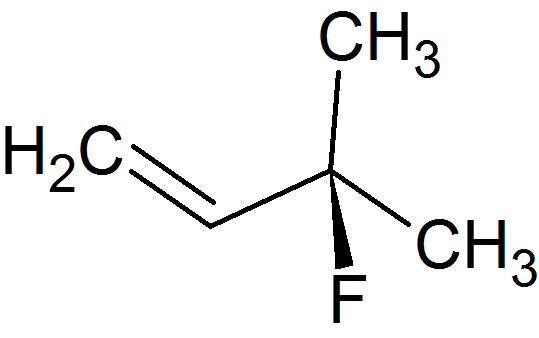
\includegraphics[width=80px]{3-fluoro-3-methyl-1-butene.png}}
\end{figure}


%Environment
Two different models of environments are applied, one with a grid of point charges and one with electric fields in X Y and Z direction. The point charge model is similar to the ChelpG model\cite{ChelpG} where random point charges are placed around the molecule at a certain distance. Here we set the number of point charges to 100.
 

%This includes perturbations from external electrostatic potentials, due to other portions of the molecule or from solvent, and inductive effects from acceptors and donors. 


% Point charges
%The magnitudes of the point charges are randomly generated using a uniform distribution between -25 and 25 amu, chosen to induce variations in the Mulliken charges on the C and H in methane and ethane that are similar to the charges induced on the methyl group in CF3CH3 (~0.2 amu).  


For each pairing of a molecular configuration with an environment, we generate expectation values of each operator that appears in the Hamiltonian (total kinetic energy, interaction of the electron density with each nucleus, and total two-electron repulsion energy).

% DATA SET
Initially the model was trained on the data set which has point charges as envirnoment. This data set has 20 configurations each in 11 different environment (1 with no environment + 10 environments). The second data set included the fields as environments, here there are the same 20 configurations with 4 enviroments(1 with no environment + 3 fields for X, Y and Z). 

We ran the original Hartree-Fock until convergence, so we have the ground truth of the steady density matrix and the energy of the given molecular system under different geometries. 
%Since we have the energy of each configuration in the dataset, we can to evaluate the computation time and also the accuracy of the result in each iteration.

% Define error
We can in turn define the error $Err$ of a density matrix as the error of matrix and the error of energy. The error of the matrix is given by $norm(\rho_i-\rho_n)$. The error of energy is given by $|E(\rho_i)-E(\rho_n)|$

Once we have the error function, we can optimize the coefficients by minimizing the error.

% 30 iterations

\subsection{Experiment settings}


%ASSUMPTION:
%Assu Coefficient (linear combination) may be similar for the same molecule \\
Although the same molecule under different geometries and different environments will have different equilibrium structures, we assume the policy that speeds up the Hartree-Fock for a certain molecule will be very similar under different settings. 

As a result, for a molecule we can train a policy under a set of instances and test it under a the other different set of instances.

After the training, we will apply these Hartree-Fock with linear combination policies on testing dataset to evaluate the performance.


%We generate a few hundred molecules dataset and divide these between a training and a test data set.
%1 etot 
%2 convergence rate (L1 norm with previous iteration)
There are twenty different geometries and three different environments. We split the whole dataset into two parts evenly. 
We use the first ten geometries to serve as the training dataset, and the reaming ten geometries as testing dataset.
%The odd numbered instances serve as training data, on the other hand the even numbered instances serve as testing data. \\

\subsection{Approach}
% Goal
The goal is to train the Hartree-Fock with linear combination policy that can reach the steady density matrix for a given molecule faster than the original Hartree-Fock.


%MENTION THE PURE LINEAR COMBINATION
One naive approach to build a good policy is always using all the density matrices we have to generate a linear combination that best approaches the final steady density matrix after one Hartree-Fock iteration.  For example, from guess density matrix $\rho_0$ we will find the best coefficient that makes the output best approaches the final objective. However, we may get some error thus the result of the first iteration is $\rho_1$.  In the next iteration, again we will try to find the linear combination $(\rho_0, \rho_1)$ that best approaches the final density matrix. we can keep doing this procedure until the output of the Hartree-Fock reaches the final steady density matrix.
Because we already know the final steady density matrix, and in each iteration we aim for the final objective directly, it's possible that we can build up a trajectory that reaches final density matrix much faster then the original process. And also we will learn a policy from it. Let's call it the "Pure Linear Combination" policy.

%SHOULD ALSO MENTIONED TWO DIFFERENT EXPERT \\
Though we already aim for the final objective in each iteration, we still can try to build up a faster trajectory from it and perhaps train the other policy which is faster than the pure linear combination one.

In the experiment, we build up two different expert's trajectories. 
One is the trajectory that has a step size of two of the "Pure Linear Combination" trajectory. The other one is the perfect trajectory which always return the final steady matrix in one iteration.

% HOW TO EVALUATE

%MENTION THE CASE THAT MAY NEVER CONVERGE \\
When iterations of Hartree-Fock converge, we can get the final steady density matrix and also the energy of the system. However, the process does not always lead to convergence. Under some strong electric field, the process may keep running and never reach convergence.

 In the experiment, we will also examine the robustness of different policies.


%What is convergence rate \\
We can plot the difference between this iteration and previous iteration to examine the rate of convergence.


%CLAIM \\ 
DAgger tries to learn a new policy by imitating the expert's demonstration. Since the policy space of the DAgger and also the Pure Linear Combination are the same, the result should be at least equal or be better to the Pure Linear Combination trajectory. 
 
Considering DAgger trains on the dataset that aggregates new dataset iteration by iteration. As the dataset growing, it adds more diversity to the dataset and may lead to a more robust policy.

\subsection{Experiment result}

%%%  

We can evaluate the performance of each policy in terms of the error and robustness. 

Figure \ref{fig:training} shows the error of each policy on training dataset for 12 iterations. The baseline is the policy that always use the average of the last two density matrices to serve as the input to the next iteration.  We can observe that all the policies seems to  converge within 10 iterations except the baseline fluctuates. The pure linear combination got the lowest error since it always aim for the final objective. On the other hand, DAgger keep aggregating datasets thus has a more diverse training data. Both the DAgger with different experts have similar performance in the first 6 iterations, and fall behinds pure linear combination after iteration 7. 

Figure \ref{fig:testing} is the result  on the testing dataset.
The baseline again fluctuates while all the other policies coverages still converges within 12 iteration. 
Pure linear combination and DAgger got pretty similar error after 12 iterations. However, the performance of linear combination fluctuates during iteration 5 - 10 while both Dagger with different experts have pretty steady decreasing trending in all 12 iteration. Dagger with the expert that has step size of 2 got a smoother curve than other policies.


%
%\begin{figure}[h!]
%  \caption{Error on training dataset}
%	\label{fig:training}
%    \includegraphics[width=220px]{Dagger_beta05_training.png}
%\end{figure}
%
%\begin{figure}[h!]
%
%  \caption{Error on testing dataset}
%  \label{fig:testing}
%    \includegraphics[width=220px]{Dagger_beta05_testing.png}
%\end{figure}


\section{CONCLUSION}

Although DAgger doesn't help to gain lower error than the pure linear combination, it does train a more robust policy which has a smooth and steady decreasing trend. It is possible that because the pure linear combination and the DAgger have the same policy spac, both using the linear combination to speed up the whole process, thus DAgger can't gain much benefit from it. However, during the training process in DAgger, it keeps aggregating the dataset hence has a more diverse training instances. This can prevent the policy from over-fitting the training dataset thus produces a more stable and smooth decreasing trend. This is a great property when dealing with large molecule or on the case which is hard to converge.


\begin{thebibliography}{9}
\bibitem{Matteus}
  Matteus Tanha, Shiva Kaul, Alex Cappiello, Geoffrey J. Gordon, David J. Yaron.
  \emph{Embedding parameters in ab initio theory to develop well-controlled approximations based on molecular similarity}.
  Technical report arXiv:1311.3440.
  
  \bibitem{DAgger}
  Stephane Ross, Geoffrey J. Gordon, J. Andrew Bagnell.
  \emph{A Reduction of Imitation Learning and Structured Prediction to No-Regret Online Learning}.
  Technical report arXiv:1011.0686, arXiv, 2011.
  
  \bibitem{DAggerCompare}
  Andreas Vlachos.
  \emph{An investigation of imitation learning algorithms for structured prediction}.
  
  \bibitem{Ross}
    Ross and J. A. Bagnell.
  \emph{Efficient reductions for imitation
learning.} Proceedings of the 13th International
Conference on Artificial Intelligence and Statistics (AISTATS),
2010.

  \bibitem{Pulay1980}
   P\'{e}ter Pulay,
  \emph{Convergence acceleration of iterative sequences. The case of SCF iteration.} Chem. Phys. Lett. 73, 393 (1980).

\end{thebibliography}

\end{document}
